\documentclass[a4paper,14pt]{article}

\usepackage{comment} % Para comentar várias linhas ao mesmo tempo

%matemática
\usepackage{amsmath}
\usepackage{amssymb}

%diagramação
\usepackage{extsizes}
\everymath{\displaystyle}
\usepackage{geometry}
\usepackage{fancyhdr}
\usepackage{multicol}
\usepackage{graphicx}
\usepackage[brazil]{babel}
\usepackage[shortlabels]{enumitem}
\usepackage{cancel}
\usepackage{textcomp}
\usepackage{tcolorbox}

%tabelas
\usepackage{array} % Para melhor formatação de tabelas
\usepackage{longtable}
\usepackage{booktabs}  % Para linhas horizontais mais bonitas
\usepackage{float}   % Para usar o modificador [H]
\usepackage{caption} % Para usar legendas em tabelas
\usepackage{wrapfig} % Para usar tabelas e figuras flutuantes
\usepackage{xcolor} % Para cores do fundo de tabelas
\usepackage{colortbl} % Para cores do fundo de tabelas

%tikzpicture
\begin{comment}
	\usepackage{tikz}
	\usepackage{scalerel}
	\usepackage{pict2e}
	\usepackage{tkz-euclide}
	\usetikzlibrary{calc}
	\usetikzlibrary{patterns,arrows.meta}
	\usetikzlibrary{shadows}
	\usetikzlibrary{external}
\end{comment}


%pgfplots
\usepackage{pgfplots}
\pgfplotsset{compat=newest}
\usepgfplotslibrary{statistics}
\usepgfplotslibrary{fillbetween}

%colours
\usepackage{xcolor}



\columnsep=2cm
\hoffset=0cm
\textwidth=8cm
\setlength{\columnseprule}{.1pt}
\setlength{\columnsep}{2cm}
\renewcommand{\headrulewidth}{0pt}
\geometry{top=1in, bottom=1in, left=0.7in, right=0.5in}

\pagestyle{fancy}
\fancyhf{}
\fancyfoot[C]{\thepage}

\begin{document}
	
	\noindent\textbf{6FMA19 - Matemática} 
	
	\begin{center}Introdução aos números negativos (Versão estudante)
	\end{center}
	
	\noindent\textbf{Nome:} \underline{\hspace{10cm}}
	\noindent\textbf{Data:} \underline{\hspace{4cm}}
	
	%\section*{Questões de Matemática}
	
	\begin{multicols}{2}
		\noindent Há vários exemplos de utilização dos números negativos: a indicação dos andares de um elevador, o extrato de uma conta bancária, a medição de temperatura, etc.
		\noindent\textsubscript{-----------------------------------------------------------------------}
		\begin{enumerate} 
			\item Imagine que, em vez de o primeiro na lista de chamada da sua sala receber o número 1, o último aluno da lista de chamada recebesse tal número. Utiliza os negativos para dizer qual seria então o número do primeiro da lista. \\\\\\\\\\\\\\\\\\\\\\\\\\\\\\\\\\\\\\\\
			\item O desenho abaixo mostra o lucro ou o prejuízo, em reais, de uma empresa de alimentos durante alguns meses. O que se pode dizer sobre esse desempenho? \\
			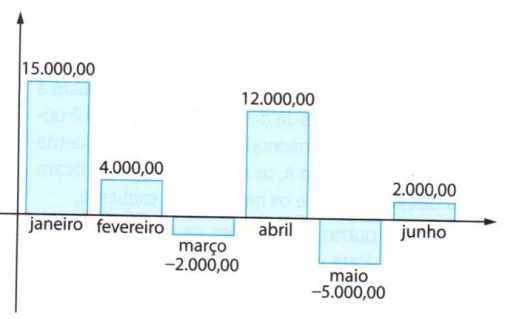
\includegraphics[width=1\linewidth]{6FMA19_imagens/imagem1} \newpage
			%69 e 70
			\item No elevador de alguns edifícios, podemos observar os botões -1, -2, e -3. O que esses botões significam? \\\\\\\\\\\\\\\\\\\\\\\\\\\\\\\\\\\\\\\\\\\\\\\\\\\\\\\\\\\\\\\\\\\\\\\\\\
			\item Analise o extrato de uma conta bancária: \\\\
			\noindent\begin{tabular}{cc}
				\rowcolor{lightgray} Saldo em conta-corrente & 450,00 \\
				\rowcolor{lightgray} Saque em caixa eletrônico & -650,00 \\
				\rowcolor{lightgray} Depósito em dinheiro & 150,00 \\
				\rowcolor{lightgray} Saldo em conta-corrente & -50,00 \\
				\rowcolor{lightgray} Cheque compensado & -100,00 \\
				\rowcolor{lightgray} Saldo em conta-corrente & -150,00 \\
			\end{tabular}
			\begin{enumerate}[a)]
				\item O que o sinal (-) na frente de 650,00 e 100,00 significa? \\\\\\\\\\\\\\\\
				\item O que o sinal (-) na frente de 150,00 significa?
			\end{enumerate}
		\end{enumerate}
		$~$ \\ $~$ \\ $~$ \\ $~$ \\ $~$ \\ $~$ \\ $~$ \\ $~$ \\ $~$ \\ $~$ \\ $~$ \\ $~$ \\ $~$ \\ $~$ \\ $~$ \\ $~$ \\ $~$ \\ $~$ \\ $~$
	\end{multicols}
\end{document}